% !TEX root= ../main.tex
\section{Inconsistencies in graph theories}
\label{sec:Inconsistencies in graph theories}
In this section we consider the graph in Figure~\ref{fig:triple_double_open_door}.
Any mention of vertices, edges and components in this section will refer to this graph.\par
\begin{figure}[!h]
  \centering
  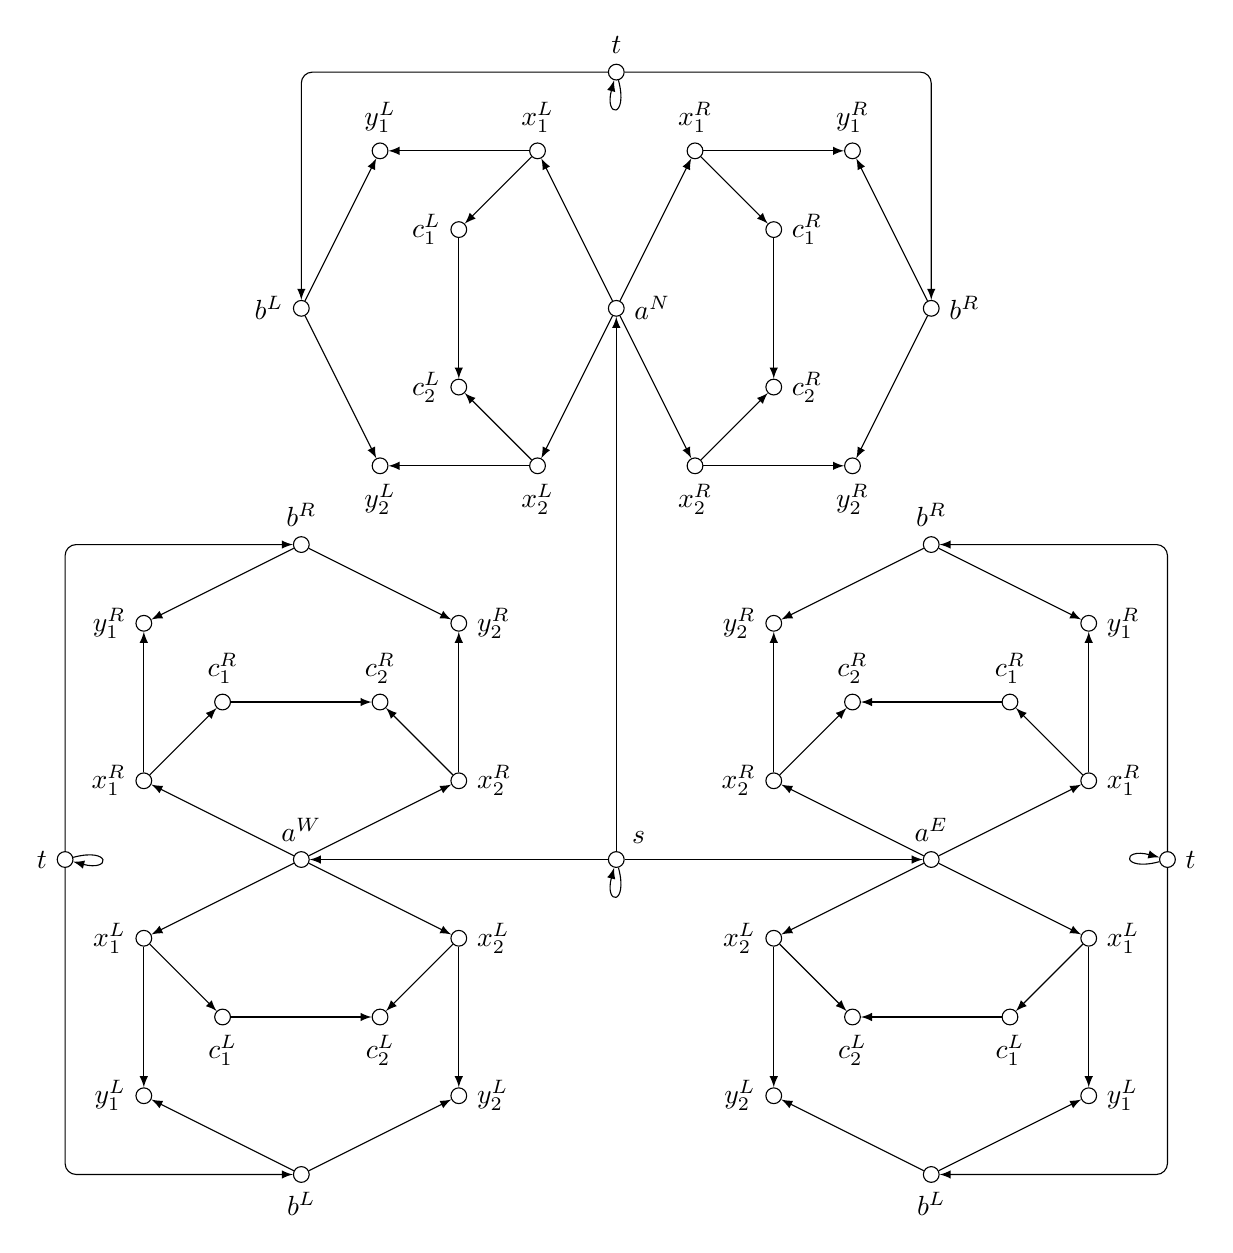
\begin{tikzpicture}
    [
    point/.style={circle,draw,inner sep=0pt,minimum size=2mm}
    ]
    \node (t) at (7,14) [point,label=above:$t$] {};
    \node (a) at (7,11) [point,label=right:$a^N$] {};
    \node (lx1) at (6,13) [point,label=above:$x^L_1$] {};
    \node (lx2) at (6,9) [point,label=below:$x^L_2$] {};
    \node (lb) at (3,11) [point,label=left:$b^L$] {};
    \node (ly1) at (4,13) [point,label=above:$y^L_1$] {};
    \node (ly2) at (4,9) [point,label=below:$y^L_2$] {};
    \node (lc1) at (5,12) [point,label=left:$c^L_1$] {};
    \node (lc2) at (5,10) [point,label=left:$c^L_2$] {};
    \draw [-latex] (a) to (lx1);
    \draw [-latex] (a) to (lx2);
    \draw [-latex] (lb) to (ly1);
    \draw [-latex] (lb) to (ly2);
    \draw [-latex] (lx1) to (ly1);
    \draw [-latex] (lx1) to (lc1);
    \draw [-latex] (lx2) to (ly2);
    \draw [-latex] (lx2) to (lc2);
    \draw [-latex] (lc1) to (lc2);
    \node (rx1) at (8,13) [point,label=above:$x^R_1$] {};
    \node (rx2) at (8,9) [point,label=below:$x^R_2$] {};
    \node (rb) at (11,11) [point,label=right:$b^R$] {};
    \node (ry1) at (10,13) [point,label=above:$y^R_1$] {};
    \node (ry2) at (10,9) [point,label=below:$y^R_2$] {};
    \node (rc1) at (9,12) [point,label=right:$c^R_1$] {};
    \node (rc2) at (9,10) [point,label=right:$c^R_2$] {};
    \draw [-latex] (a) to (rx1);
    \draw [-latex] (a) to (rx2);
    \draw [-latex] (rb) to (ry1);
    \draw [-latex] (rb) to (ry2);
    \draw [-latex] (rx1) to (ry1);
    \draw [-latex] (rx1) to (rc1);
    \draw [-latex] (rx2) to (ry2);
    \draw [-latex] (rx2) to (rc2);
    \draw [-latex] (rc1) to (rc2);
    \draw [-latex, rounded corners] (t) -| (lb);
    \draw [-latex, rounded corners] (t) -| (rb);
    \draw [-latex, loop below] (t) to (t);

    \node (wt) at (0,4) [point,label=left:$t$] {};
    \node (wa) at (3,4) [point,label=above:$a^W$] {};
    \node (wlx1) at (1,3) [point,label=left:$x^L_1$] {};
    \node (wlx2) at (5,3) [point,label=right:$x^L_2$] {};
    \node (wlb) at (3,0) [point,label=below:$b^L$] {};
    \node (wly1) at (1,1) [point,label=left:$y^L_1$] {};
    \node (wly2) at (5,1) [point,label=right:$y^L_2$] {};
    \node (wlc1) at (2,2) [point,label=below:$c^L_1$] {};
    \node (wlc2) at (4,2) [point,label=below:$c^L_2$] {};
    \draw [-latex] (wa) to (wlx1);
    \draw [-latex] (wa) to (wlx2);
    \draw [-latex] (wlb) to (wly1);
    \draw [-latex] (wlb) to (wly2);
    \draw [-latex] (wlx1) to (wly1);
    \draw [-latex] (wlx1) to (wlc1);
    \draw [-latex] (wlx2) to (wly2);
    \draw [-latex] (wlx2) to (wlc2);
    \draw [-latex] (wlc1) to (wlc2);
    \node (wrx1) at (1,5) [point,label=left:$x^R_1$] {};
    \node (wrx2) at (5,5) [point,label=right:$x^R_2$] {};
    \node (wrb) at (3,8) [point,label=above:$b^R$] {};
    \node (wry1) at (1,7) [point,label=left:$y^R_1$] {};
    \node (wry2) at (5,7) [point,label=right:$y^R_2$] {};
    \node (wrc1) at (2,6) [point,label=above:$c^R_1$] {};
    \node (wrc2) at (4,6) [point,label=above:$c^R_2$] {};
    \draw [-latex] (wa) to (wrx1);
    \draw [-latex] (wa) to (wrx2);
    \draw [-latex] (wrb) to (wry1);
    \draw [-latex] (wrb) to (wry2);
    \draw [-latex] (wrx1) to (wry1);
    \draw [-latex] (wrx1) to (wrc1);
    \draw [-latex] (wrx2) to (wry2);
    \draw [-latex] (wrx2) to (wrc2);
    \draw [-latex] (wrc1) to (wrc2);
    \draw [-latex, rounded corners] (wt) |- (wlb);
    \draw [-latex, rounded corners] (wt) |- (wrb);
    \draw [-latex, loop right] (wt) to (wt);

    \node (et) at (14,4) [point,label=right:$t$] {};
    \node (ea) at (11,4) [point,label=above:$a^E$] {};
    \node (elx1) at (13,3) [point,label=right:$x^L_1$] {};
    \node (elx2) at (9,3) [point,label=left:$x^L_2$] {};
    \node (elb) at (11,0) [point,label=below:$b^L$] {};
    \node (ely1) at (13,1) [point,label=right:$y^L_1$] {};
    \node (ely2) at (9,1) [point,label=left:$y^L_2$] {};
    \node (elc1) at (12,2) [point,label=below:$c^L_1$] {};
    \node (elc2) at (10,2) [point,label=below:$c^L_2$] {};
    \draw [-latex] (ea) to (elx1);
    \draw [-latex] (ea) to (elx2);
    \draw [-latex] (elb) to (ely1);
    \draw [-latex] (elb) to (ely2);
    \draw [-latex] (elx1) to (ely1);
    \draw [-latex] (elx1) to (elc1);
    \draw [-latex] (elx2) to (ely2);
    \draw [-latex] (elx2) to (elc2);
    \draw [-latex] (elc1) to (elc2);
    \node (erx1) at (13,5) [point,label=right:$x^R_1$] {};
    \node (erx2) at (9,5) [point,label=left:$x^R_2$] {};
    \node (erb) at (11,8) [point,label=above:$b^R$] {};
    \node (ery1) at (13,7) [point,label=right:$y^R_1$] {};
    \node (ery2) at (9,7) [point,label=left:$y^R_2$] {};
    \node (erc1) at (12,6) [point,label=above:$c^R_1$] {};
    \node (erc2) at (10,6) [point,label=above:$c^R_2$] {};
    \draw [-latex] (ea) to (erx1);
    \draw [-latex] (ea) to (erx2);
    \draw [-latex] (erb) to (ery1);
    \draw [-latex] (erb) to (ery2);
    \draw [-latex] (erx1) to (ery1);
    \draw [-latex] (erx1) to (erc1);
    \draw [-latex] (erx2) to (ery2);
    \draw [-latex] (erx2) to (erc2);
    \draw [-latex] (erc1) to (erc2);
    \draw [-latex, rounded corners] (et) |- (elb);
    \draw [-latex, rounded corners] (et) |- (erb);
    \draw [-latex, loop left] (et) to (et);

    \node (s) at (7,4) [point,label=above right:$s$] {};
    \draw [-latex] (s) to (a);
    \draw [-latex] (s) to (wa);
    \draw [-latex] (s) to (ea);
    \draw [-latex,loop below] (s) to (s);
  \end{tikzpicture}
  \caption{}
  \label{fig:triple_double_open_door}
\end{figure}
The graph contains 3 copies of the graph from Figure~\ref{fig:double_open_door};
one northern (N), one western (W) and one eastern (E).
We call these \textit{components}.
Every vertex in the graph is contained within exactly one component, except the vertex $s$ which is not inside any component.

The first thing to notice is that the graph is inconsistent;
the proof of $\ol{a}$ from Figure~\ref{fig:unary_nand_proof} can be applied to each component in the above graph, giving us the provability of $\ol{a^N}$, $\ol{a^W}$ and $\ol{a^E}$.
From here, the inconsistency proof is trivial;
shown in Figure~\ref{fig:triple_double_open_door_proof}.\par
\begin{figure}[!h]
  \centering
  \begin{prooftree*}
    \Hypo{\ol{s}}
    \Hypo{\dots}
    \Infer[]1{\ol{a^N}}
    \Hypo{\dots}
    \Infer[]1{\ol{a^W}}
    \Hypo{\dots}
    \Infer[]1{\ol{a^E}}
    \Infer[right label=$sa^Na^Wa^E$]4{\varnothing}
  \end{prooftree*}
  \caption{}
  \label{fig:triple_double_open_door_proof}
\end{figure}
We will ultimately show that the inconsistency is not binary-derivable, but first we prove some lemmata.
\begin{lemma}
  Let the vertices $u$ and $v$ be from different components in the graph.
  If $\ol{uv}$ is binary-derivable, then its proof contains either $\ol{a^N}$, $\ol{a^W}$ or $\ol{a^E}$.
  \label{thm:uv_proof_contains_a}
\end{lemma}
\begin{proof}
  Base Case:
  No axiom $\ol{uv}$ exists such that $u$ and $v$ are vertices from different components, so our claim vacuously holds.

  Induction Step:
  Suppose we have a binary proof of $\ol{uv}$ where $u$ and $v$ are from different components.
  The premise of the last proof step must contain at least one binary NAND-clause containing $u$ and one containing $v$.\par
  \begin{figure}[!h]
    \centering
    \begin{prooftree*}
      \Hypo{\ol{u\dots}}
      \Hypo{\ol{v\dots}}
      \Hypo{\dots}
      \Infer[]3{\ol{uv}}
    \end{prooftree*}
    \caption{}
    \label{fig:proof_scheme_uv}
  \end{figure}
  If either $u$ or $v$ are in a clause together with a vertex from a component different from their own, we get from the induction hypothesis that their proof must contain either $\ol{a^N}$, $\ol{a^W}$ or $\ol{a^E}$, so we are done.

  Otherwise, $u$ and $v$ are each either in a clause together with the vertex $s$ or a vertex from their own component.
  Both of these cases results in having to use the OR-clause $sa^Na^Wa^E$ in the last proof step, since it is the only OR-clause containing $s$ and the only OR-clause containing vertices from different components.
  The premise therefore contains two additional NAND-clauses; one of them containing the $a$-vertex of the component not containing $u$ or $v$ - lets call it $a^t$.

  Figure~\ref{fig:proof_example_uv} contains examples of two possible cases.\par
  \begin{figure}[!h]
    \centering
    \begin{prooftree}
      \Hypo{\ol{s\dots}}
      \Hypo{\ol{ua^N}}
      \Hypo{\ol{va^W}}
      \Hypo{\ol{a^E\dots}}
      \Infer[right label=$sa^Na^Wa^E$]4{\ol{uv}}
    \end{prooftree}
    \hspace{5mm}
    \begin{prooftree}
      \Hypo{\ol{us}}
      \Hypo{\ol{va^N}}
      \Hypo{\ol{a^W\dots}}
      \Hypo{\ol{a^E\dots}}
      \Infer[right label=$sa^Na^Wa^E$]4{\ol{uv}}
    \end{prooftree}
    \caption{}
    \label{fig:proof_example_uv}
  \end{figure}
  If the clause containing $a^t$ is unary, we are done.
  If it is binary, it must either contain $u$ or $v$ in order to give $\ol{uv}$ in the conclusion, and since $a^t$ is in a component different from both $u$ and $v$, the induction hypothesis gives us the claim.

  The proof must therefore contain either $\ol{a^N}$, $\ol{a^W}$ or $\ol{a^E}$.
\end{proof}
\begin{lemma}
  $\ol{a^N}$, $\ol{a^W}$ and $\ol{a^E}$ are not binary-derivable.
  \label{thm:non_binary_derivable_a}
\end{lemma}
\begin{proof}
  We prove it by structural induction over the complexity of the proof tree.

  Base Case:
  Neither $\ol{a^N}$, $\ol{a^W}$ nor $\ol{a^E}$ are axioms, so the claim vacuously holds.

  Induction step:
  Suppose we have a binary proof of $\ol{a}$, where $a$ is either $a^N$, $a^W$ or $a^E$.
  The vertices within the same component as the one containing $a$ will be referred to as \textit{internal} vertices, while the vertices within the two other components will be referred to as \textit{external} vertices.
  Note that since $s$ is not inside any component, it is neither internal nor external.

  First, since the proof is binary, we get from our induction hypothesis that neither $\ol{a^N}$, $\ol{a^W}$ nor $\ol{a^E}$ appears in it.

  We get from Lemma~\ref{thm:a_not_binary_derivable} that $\ol{a}$ is not binary-derivable if one is using internal vertices only, so the binary proof must use vertices outside the component containing $a$; either the $s$-vertex or external vertices.

  If it uses $s$, consider the last proof step with $s$ in the premise.
  The OR-clause used in this proof step must be $sa^Na^Wa^E$, being the only OR-clause containing $s$ and thus the only clause able to remove it.
  This OR-clause contains 4 vertices, so the premise must contain 3 additional NAND-clauses;
  one containing $a^N$, one containing $a^W$ and one containing $a^E$.

  We get the following restrictions on these 3 NAND-clauses.
  \begin{itemize}
    \item None of them can be unary, from the induction hypothesis.
    \item None of them can be binary and contain $s$, since that would give an $s$ in the conclusion, contradicting our assumption of this being the last proof step with $s$ in the premise.
    \item None of them can be binary and contain vertices from two different components, from the induction hypothesis and Lemma~\ref{thm:uv_proof_contains_a}.
  \end{itemize}
  The 3 additional NAND-clauses must therefore all contain a second vertex $p$ from their own component.

  Since the three components are disjoint, these three $p$-vertices are different, making the conclusion of the proof step non-binary, contradicting our original assumption of the proof being binary.

  If the proof does \textit{not} contain $s$, then it uses external vertices.
  Consider the last proof step containing external vertices in the premise.
  This proof step removes these vertices and conclude with some clause only internal vertices.
  The premise must contain, in addition to all the clauses with external vertices, at least one binary NAND-clause with an internal vertex, in order to make the conclusion non-empty.
  This clause cannot contain any external vertices, from Lemma~\ref{thm:uv_proof_contains_a} and the induction hypothesis, so it must be a clause with two internal vertices.
  The OR-clause used in the proof step must therefore contain both external vertices and at least one internal vertex.
  Since $sa^Na^Wa^E$ is the only OR-clause containing vertices from different components, it is the only option, but we just assumed that $s$ is not in this proof, so we reach a contradiction.

  $\ol{a}$ is thus not binary-derivable.
\end{proof}
\begin{corollary}
  $\ol{x^1x^2}$ is not binary-derivable.
  \label{thm:non_binary_derivable_uv}
\end{corollary}
\begin{proof}
  We get this directly from Lemma 1 and Lemma 2.
\end{proof}

\begin{theorem}
  $\varnothing$ is not binary-derivable.
  \label{thm:non_binary_derivable_paradox}
\end{theorem}
\begin{proof}
  Assume we have a binary proof of $\varnothing$;
  proof must contain $\ol{s}$.
  Consider the last proof step with $s$ in the premise:
  This proof step must remove $s$ and thus use the OR-claus e$sa^Na^Wa^E$.
  Premise must contain 3 additional NAND-clauses;
  one containing $a^N$, one containing $a^W$ and one containing $a^E$.
  \begin{itemize}
    \item None of them can contain $s$, since that would give an $s$ in the conclusion.
    \item None of them can be unary, from Lemma 2.
    \item None of them can contain a second vertex from another component, from Corollary 3.
  \end{itemize}
  The 3 additional NAND-clauses must therefore all contain a second vertex from its own component,
  making the conclusion non-binary, contradiction our original assumption.

  $\varnothing$ is therefore not binary-derivable.
\end{proof}
